% meta.concepts: truss, method of sections
% meta.tags: 
% acknowledge: Peter Seiler & Luke Melander graciously shared Spring 2019 course material
% source: 2019 P. Seiler AEM2011 HW 8

Considering the truss shown in Fig. 2, answer the following questions:
\begin{enumerate}
  \item Show that the truss is stable (\textit{i.e. static}).
  \item Find the fices in members cd, cg, and gh.
\end{enumerate}

\begin{figure}[ht!]
  \centering
  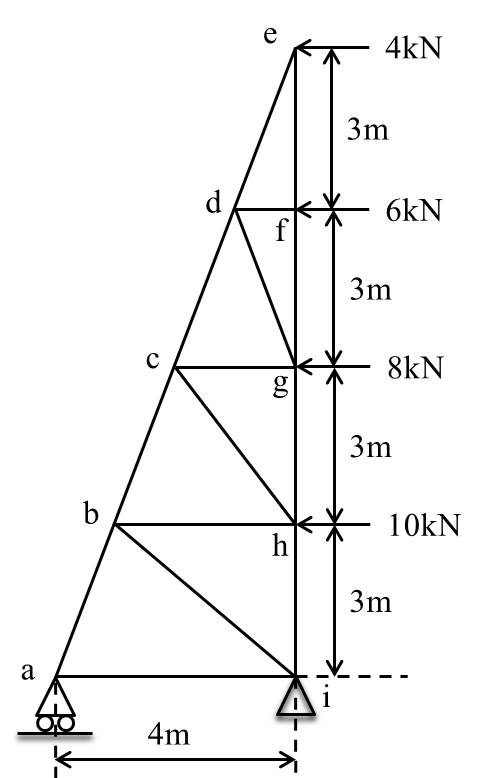
\includegraphics[width=0.5\textwidth,
	           height=0.4\textheight,
		   keepaspectratio]{fig.png}
  \caption*{Schematic of Truss}
\end{figure}

\iftoggle{flagSoln}{%
\vspace{.5cm}
\rule{\textwidth}{.4pt}
\vspace{.5cm}
\textbf{Solution:}
\begin{figure}[ht!]
  \centering
  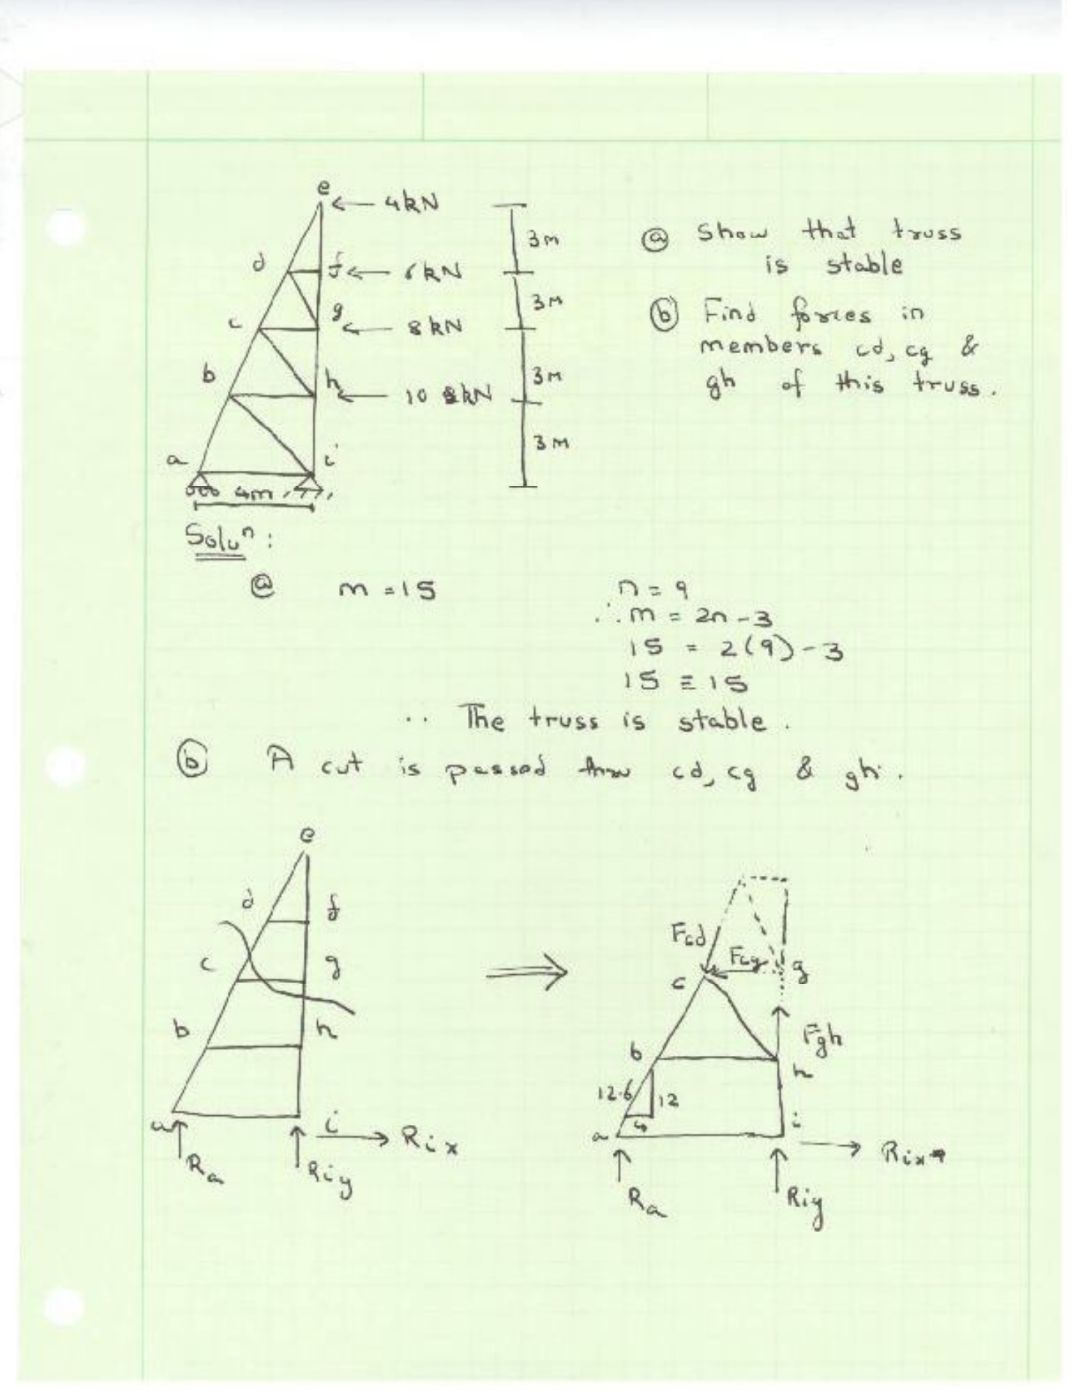
\includegraphics[width=0.4\textwidth,
	           height=0.4\textheight,
		   keepaspectratio]{solna.png}
  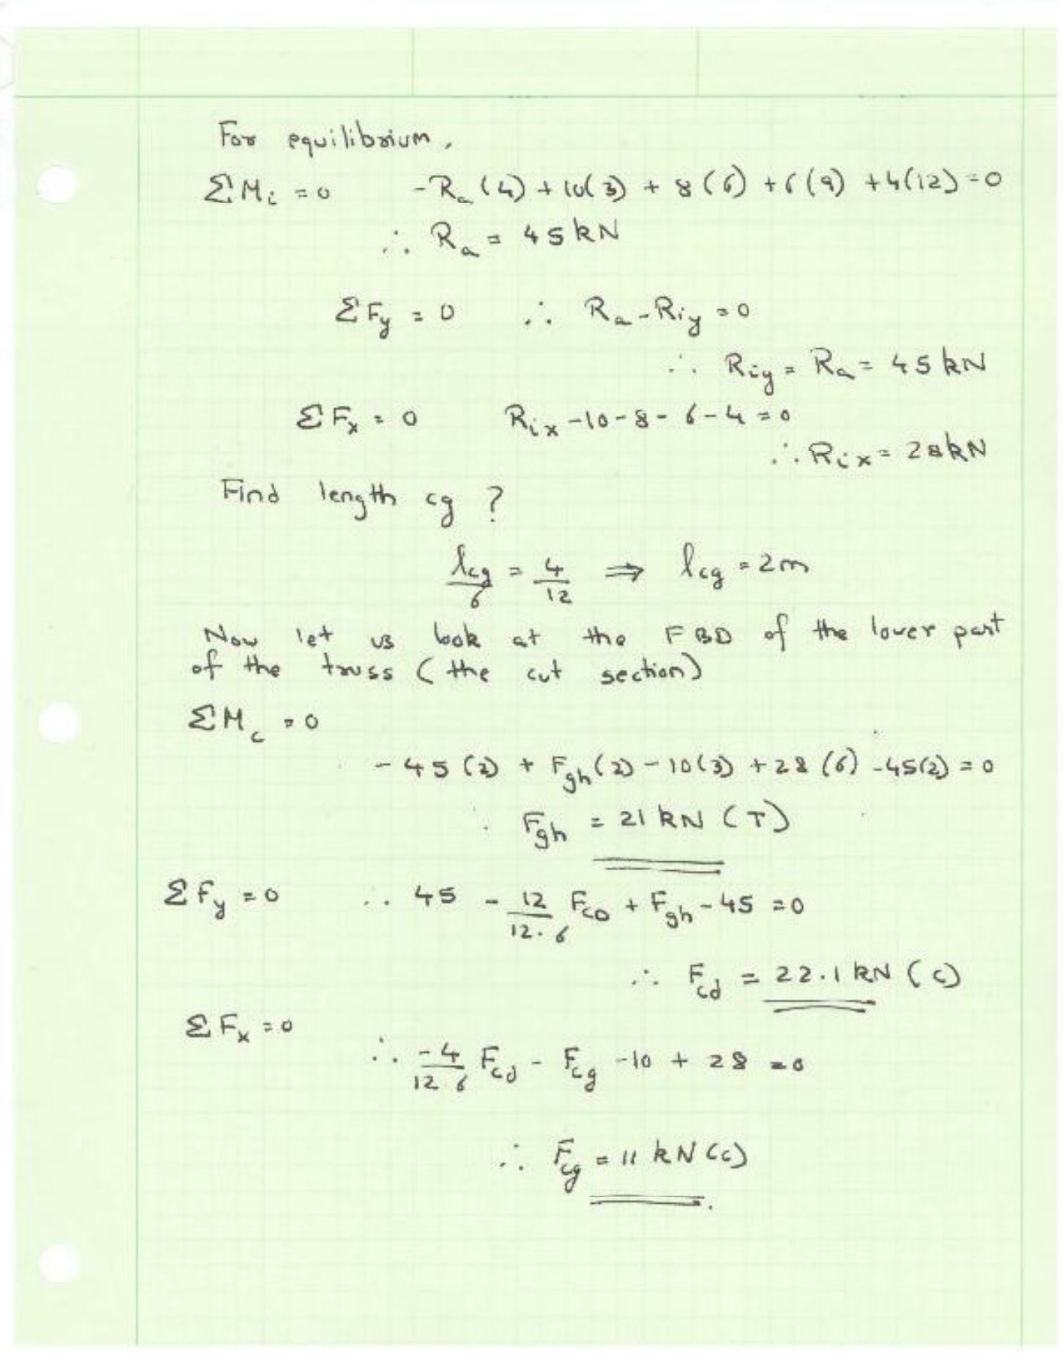
\includegraphics[width=0.4\textwidth,
	           height=0.4\textheight,
		   keepaspectratio]{solnb.png}
\end{figure}
}{%
}%
